%Este trabalho está licenciado sob a Licença Atribuição-CompartilhaIgual 4.0 Internacional Creative Commons. Para visualizar uma cópia desta licença, visite http://creativecommons.org/licenses/by-sa/4.0/deed.pt_BR ou mande uma carta para Creative Commons, PO Box 1866, Mountain View, CA 94042, USA.

\chapter{Derivação}\label{cap_deriv}
\thispagestyle{fancy}

Neste capítulo, discutimos os métodos fundamentais de derivação numérica de funções.

\section{Derivadas de primeira ordem}\label{cap_deriv_sec_df}

A derivada de uma função $f$ num ponto $x$ é, por definição,
\begin{equation}
  f'(x) = \lim_{h\to 0} \frac{f(x+h) - f(x)}{h}.
\end{equation}
Assim sendo e assumindo $h>0$\footnote{Para fixar notação, assumiremos $h>0$ ao longo deste capítulo.} próximo de zero, temos que $f'(x)$ pode ser aproximada pela razão fundamental, i.e.
\begin{equation}\label{eq_razao_fundamental}
  f'(x) \approx \underbrace{\frac{f(x+h) - f(x)}{h}}_{D_hf(x)}.
\end{equation}
Analisando a Figura~\ref{fig:intro_deriv} vemos que, geometricamente, isto é análogo a aproximar a declividade da reta tangente ao gráfico da função $f$ no ponto $(x,f(x))$ pela declividade da reta secante ao gráfico da função $f$ pelos pontos $(x,f(x))$ e $(x+h,f(x+h))$.

\begin{figure}[hp]
  \centering
  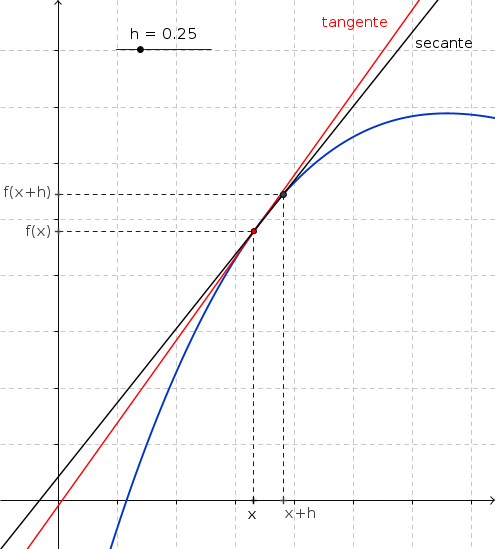
\includegraphics[width=0.7\textwidth]{cap_deriv/dados/fig_intro_deriv/fig_intro_deriv}
  \caption{Interpretação geométrica da aproximação da derivada pela razão fundamental. Veja no \href{https://github.com/phkonzen/notas/blob/master/src/MatematicaNumerica/cap_deriv/dados/fig_intro_deriv/fig_intro_deriv.ggb}{Geogebra}.}
  \label{fig:intro_deriv}
\end{figure}

\begin{ex}\label{ex_intro_deriv}
  A derivada de $f(x) = \sen(x)$ no ponto $\pi/3$ é $f'(\pi/3) = \cos(\pi/3)=0,5$. Agora, usando a aproximação pela razão fundamental~\eqref{eq_razao_fundamental}, temos
  \begin{align}
    f'\left(\frac{\pi}{3}\right) \approx D_hf(x) &= \frac{f\left(\frac{\pi}{3}+h\right)-f\left(\frac{\pi}{3}\right)}{h}\\
          &= \frac{\sen\left(\frac{\pi}{3}\right)-\sen\left(\frac{\pi}{3}\right)}{h}. 
  \end{align}
Na Tabela~\ref{tab:ex_intro_deriv} temos os valores desta aproximação para diferentes escolhas da passo $h$.

\begin{table}[hp]
  \centering
  \begin{tabular}{l|c}
    $h$ & $Df(\pi/3)$ \\ \hline
    $10^{-1}$ & $4,55902\E-1$ \\
    $10^{-2}$ & $4,95662\E-1$ \\
    $10^{-3}$ & $4,99567\E-1$ \\
    $10^{-5}$ & $4,99996\E-1$ \\
    $10^{-10}$ & $5.00000\E-1$ \\\hline
  \end{tabular}
  \caption{Valores aproximados da derivada de $f(x)=\sen(x)$ no ponto $x=\pi/6$ usado a expressão~\eqref{eq_razao_fundamental}.}
  \label{tab:ex_intro_deriv}
\end{table}
\end{ex}

A aproximação~\eqref{eq_razao_fundamental} é uma \emph{fórmula de diferenças finitas}\index{diferenças finitas}. Existem várias aproximações deste tipo que podem ser derivadas. Além disso, tais derivações nos permitem estimar o erro na utilização de tais fórmulas para a aproximação de derivadas. Na sequência, discutiremos o desenvolvimento de fórmulas de diferenças finitas usando polinômios de Taylor.

\subsection{Desenvolvimento por polinômio de Taylor}

Aqui, discutimos a obtenção de fórmulas de diferenças finitas via polinômio de Taylor.

\subsubsection{Diferenças finitas progressiva de ordem $h$}

A aproximação por polinômio de Taylor de grau 1 de uma dada função $f$ em torno no ponto $x$ é
\begin{equation}\label{eq:poli_Taylor_grau_1}
  f(x+h) = f(x) + hf'(x) + O(h^2).
\end{equation}
Agora, isolando $f'(x)$, obtemos
\begin{equation}
  f'(x) = \frac{f(x+h) - f(x)}{h} + O(h).
\end{equation}
Isto nos fornece a chamada fórmula de diferenças finitas progressiva de ordem $h$\index{diferenças finitas!progressiva de ordem $h$}
\begin{equation}\label{eq:dfp_h}
  D_{+,h}f(x) := \frac{f(x+h) - f(x)}{h}.
\end{equation}
Observemos que a ordem da fórmula se refere a ordem do erro de truncamento com respeito ao passo $h$.

\begin{ex}\label{ex:dfp_h}
  Consideremos o problema de aproximar a derivada da função $f(x) = \sen(x)$ no ponto $\pi/3$. Usando a fórmula de diferenças finitas progressiva de ordem $h$ obtemos
  \begin{align}
    f'\left(\frac{\pi}{3}\right) \approx D_{+,h}f(x) &= \frac{f\left(\frac{\pi}{3}+h\right)-f\left(\frac{\pi}{3}\right)}{h}\\
          &= \frac{\sen\left(\frac{\pi}{3}+h\right)-\sen\left(\frac{\pi}{3}\right)}{h}. 
  \end{align}
Na Tabela~\ref{tab:ex_dfp_h} temos os valores desta aproximação para diferentes escolhas de $h$, bem como, o erro absoluto da aproximação de $f'(\pi/3)$ por $D_{+,h}f(\pi/3)$.

\begin{table}[h!]
  \centering
  \caption{Resultados referente ao Exemplo~\ref{ex:dfp_h}.}
  \begin{tabular}{l|c|c}
    $h$ & $D_{+,h}f(\pi/3)$ & $|f'(\pi/3)-D_{+,h}f(\pi/3)|$\\ \hline
    $10^{-1}$ & $4,55902\E-1$ & $4,4\E-2$ \\
    $10^{-2}$ & $4,95662\E-1$ & $4,3\E-3$ \\
    $10^{-3}$ & $4,99567\E-1$ & $4,3\E-4$ \\
    $10^{-5}$ & $4,99996\E-1$ & $4,3\E-6$ \\
    $10^{-10}$ & $5.00000\E-1$ & $4,1\E-8$ \\\hline
  \end{tabular}
  \label{tab:ex_dfp_h}
\end{table}
\end{ex}

\begin{obs}
  No exemplo acima (Exemplo~\ref{ex:dfp_h}), podemos observar que o erro absoluto na aproximação de $f'(x)$ por $D_{+,h}f(x)$ decresce conforme a ordem do erro de truncamento para valores moderados de $h$ (veja, Tabela~\ref{tab:ex_dfp_h}). Agora, para valores de $h$ muito pequenos (por exemplo, $h=10^{-10}$), o erro $|f'(x)-D_{+,h}f(x)|$ não segue mais a tendência de decaimento na mesma do de truncamento. Isto se deve a dominância dos erros de arredondamento para valores muito pequenos de $h$. 

  Para mais informações sobre o comportamento do erro de arredondamento em fórmulas de diferenças finitas, veja, por exemplo, \href{https://www.ufrgs.br/reamat/CalculoNumerico/livro-oct/dn-diferencas_finitas.html}{REAMAT - Cálculo Numérico - Versão GNU Octave - Diferenças Finitas - Erro de arredondamento}.
\end{obs}

\subsubsection{Diferenças finitas regressiva de ordem $h$}

Substituindo $h$ por $-h$ na equação~\eqref{eq:poli_Taylor_grau_1}, obtemos
\begin{equation}
  f(x-h) = f(x) - hf'(x) + O(h^2),
\end{equation}
donde obtemos a fórmula de diferenças finitas regressiva de ordem $h$\index{diferenças finitas!regressiva de ordem $h$}
\begin{equation}\label{eq:dfr_h}
  D_{-,h}f(x) = \frac{f(x) - f(x-h)}{h}.
\end{equation}

\begin{ex}\label{ex:dfr_h}
  Consideremos o problema de aproximar a derivada da função $f(x) = \sen(x)$ no ponto $\pi/3$. Usando a fórmula de diferenças finitas regressiva de ordem $h$ obtemos
  \begin{align}
    f'\left(\frac{\pi}{3}\right) \approx D_{-,h}f(x) &= \frac{f\left(\frac{\pi}{3}\right)-f\left(\frac{\pi}{3}-h\right)}{h}\\
          &= \frac{\sen\left(\frac{\pi}{3}\right)-\sen\left(\frac{\pi}{3}-h\right)}{h}. 
  \end{align}
Na Tabela~\ref{tab:ex_dfr_h} temos os valores desta aproximação para diferentes escolhas de $h$, bem como, o erro absoluto da aproximação de $f'(\pi/3)$ por $D_{-,h}f(\pi/3)$.

\begin{table}[h!]
  \centering
  \caption{Resultados referente ao Exemplo~\ref{ex:dfr_h}.}
  \begin{tabular}{l|c|c}
    $h$ & $D_{-,h}f(\pi/3)$ & $|f'(\pi/3)-D_{-,h}f(\pi/3)|$\\ \hline
    $10^{-1}$ & $5,42432\E-1$ & $4,2\E-2$ \\
    $10^{-2}$ & $5,04322\E-1$ & $4,3\E-3$ \\
    $10^{-3}$ & $5,00433\E-1$ & $4,3\E-4$ \\
    $10^{-5}$ & $5,00004\E-1$ & $4,3\E-6$ \\
    $10^{-10}$ & $5.00000\E-1$ & $4,1\E-8$ \\\hline
  \end{tabular}
  \label{tab:ex_dfr_h}
\end{table}
\end{ex}

\subsubsection{Diferenças finitas central de ordem $h^2$}

Usando o polinômio de Taylor de grau 2 para aproximar a função $f(x)$ em torno de $x$, obtemos
\begin{align}
  f(x+h) &= f(x) + hf'(x) + \frac{h}{2}f''(x) + O(h^3)\\
  f(x-h) &= f(x) - hf'(x) + \frac{h}{2}f''(x) + O(h^3).
\end{align}
Então, subtraindo esta segunda equação da primeira, temos
\begin{equation}
  f(x+h)-f(x-h) = 2hf(x) + O(h^3).
\end{equation}
Agora, isolando $f(x)$
\begin{equation}
  f(x) = \frac{f(x+h)-f(x-h)}{2h} + O(h^2),
\end{equation}
o que nos fornece a chamada fórmula de diferenças finitas central de ordem $h^2$\index{diferenças finitas!central de ordem $h^2$}
\begin{equation}\label{eq:dfc_h2}
  D_{0,h^2}f(x) := \frac{f(x+h)-f(x-h)}{2h}.
\end{equation}

\begin{ex}\label{ex:dfc_h2}
  Consideremos o problema de aproximar a derivada da função $f(x) = \sen(x)$ no ponto $\pi/3$. Usando a fórmula de diferenças finitas central de ordem $h^2$ obtemos
  \begin{align}
    f'\left(\frac{\pi}{3}\right) \approx D_{0,h^2}f(x) &= \frac{f\left(\frac{\pi}{3}+h\right)-f\left(\frac{\pi}{3}-h\right)}{2h}\\
          &= \frac{\sen\left(\frac{\pi}{3}+h\right)-\sen\left(\frac{\pi}{3}-h\right)}{2h}. 
  \end{align}

\begin{table}[h!]
  \centering
  \caption{Resultados referente ao Exemplo~\ref{ex:dfc_h2}.}
  \begin{tabular}{l|c|c}
    $h$ & $D_{0,h}f(\pi/3)$ & $|f'(\pi/3)-D_{0,h^2}f(\pi/3)|$\\ \hline
    $10^{-1}$ & $4,99167\E-1$ & $8,3\E-04$ \\
    $10^{-2}$ & $4,99992\E-1$ & $8,3\E-06$ \\
    $10^{-3}$ & $5,00000\E-1$ & $8,3\E-08$ \\
    $10^{-5}$ & $5,00000\E-1$ & $8,3\E-10$ \\
    $10^{-10}$ & $5.00000\E-1$ & $7,8\E-12$ \\\hline
  \end{tabular}
  \label{tab:ex_dfc_h2}
\end{table}

Na Tabela~\ref{tab:ex_dfc_h2} temos os valores desta aproximação para diferentes escolhas de $h$, bem como, o erro absoluto da aproximação de $f'(\pi/3)$ por $D_{0,h^2}f(\pi/3)$.

\end{ex}


\subsection*{Exercícios}

\emconstrucao

\section{Diferenças finitas por polinômios interpoladores}

Aqui, discutimos a obtenção de fórmulas de diferenças finitas por polinômios interpoladores. Seja $p(x)$ o polinômio interpolador dos pontos $\{(x_i,f(x_i))\}_{i=1}^{n+1}$ de uma dada função $f(x)$, com $x_1 < x_2 < \cdots < x_{n+1}$. Então, pelo teorema de Lagrange temos
\begin{equation}
  f(x) = p(x) + R_{n+1}(x),
\end{equation}
onde $R(x)$ é o erro na aproximação de $f(x)$ por $p(x)$ e tem a forma
\begin{equation}
  R_{n+1}(x) = \frac{f^{(n+1)}(\xi)}{(n+1)!}\prod_{j=1}^{n+1}(x-x_j).
\end{equation}
onde $\xi = \xi(x)$.

Deste modo, a ideia para obtermos as fórmulas de diferenças é aproximarmos $f'(x)$ por $p'(x)$. Entretanto, isto nos coloca a questão de estimarmos o erro $|f'(x) - p'(x)|$. Por sorte temos os seguinte teorema.

\begin{teo}\label{teo:erro_de_Lagrange_deriv}
  Seja $p(x)$ o polinômio interpolador de uma dada função $f(x)$ pelo pontos $\{(x_i, f(x_i))\}_{i=1}^{n+1}$, com $x_1<x_2<\cdots<x_{n+1}$. Se $f(x)$ é $(n+1)$ continuamente diferenciável, então o resíduo $R_{n+1}^{(k)}(x) = f^{(k)}(x) - p^{(k)}(x)$ é
  \begin{equation}
    R_{n+1}^{(k)} = \frac{f^{(n+1)}(\eta) }{(n+1-k)!}\prod_{j=1}^{n+1-k}(x-\xi_j),
  \end{equation}
onde $\xi_j$ é um ponto tal que $x_j < \xi_j < x_{j+k}$, $j=1, 2, \dotsc, n+1+k$, e $\eta = \eta(x)$ é algum ponto no intervalo de extremos $x$ e $\xi_j$. 
\end{teo}
\begin{dem}
  Veja \cite[Ch.6, Sec.5]{Isaacson1994a}.
\end{dem}

\subsection{Fórmulas de dois pontos}

Seja $p(x)$ o polinômio interpolador de Lagrange de $f(x)$ pelos pontos $(x_1, f(x_1))$ e $(x_2, f(x_2))$, com $x_1 < x_2$, i.e.
\begin{align}
  f(x) &= p(x) + R_{2}(x)\\
  &= f(x_1)\frac{x-x_2}{x_1-x_2} + f(x_2)\frac{x-x_1}{x_2-x_1} + R_2(x).
\end{align}
Denotando $h=x_2-x_1$, temos
\begin{equation}
  f(x) = f(x_1)\frac{x-x_2}{-h} + f(x_2)\frac{x-x_1}{h} + R_2(x).
\end{equation}
e, derivando com respeito a $x$
\begin{equation}
  f'(x) = \frac{f(x_2)-f(x_1)}{h} + R_2^{(1)}(x),
\end{equation}
onde $ R_2^{(1)}(x)$ é dado conforme o teorema~\ref{teo:erro_de_Lagrange_deriv}.

Agora, escolhendo $x=x_1$, temos $x_2 = x_1 + h = x + h$ e, obtemos a fórmula de diferenças finitas progressiva de ordem $h$
\begin{equation}
  f(x) = \underbrace{\frac{f(x+h) - f(x)}{h}}_{D_{+,h}f(x)} + O(h).
\end{equation}

Se escolhermos $x=x_2$, temos $x_1 = x_2 - h = x - h$, obtemos a fórmula de diferenças finitas regressiva de ordem $h$
\begin{equation}
  f(x) = \underbrace{\frac{f(x) - f(x-h)}{h}}_{D_{-,h}f(x)} + O(h).
\end{equation}

\subsubsection{Fórmulas de três pontos}

Para obtermos fórmulas de diferenças finitas de três pontos consideramos o polinômio interpolador de Lagrange de $f(x)$ pelos pontos $(x_1, f(x_1))$, $(x_2, f(x_2))$ e $(x_3, f(x_3))$, $x_1<x_2<x_3$, i.e.
\begin{align}
  f(x) &= f(x_1)\frac{(x-x_2)(x-x_3)}{(x_1-x_2)(x_1-x_3)} \\
  &+ f(x_2)\frac{(x-x_1)(x-x_3)}{(x_2-x_1)(x_2-x_3)} \\
  &+ f(x_3)\frac{(x-x_1)(x-x_2)}{(x_3-x_1)(x_3-x_2)} + R_3(x).
\end{align}
Derivando em relação a $x$, obtemos
\begin{align}\label{eq:aux_deriv1}
  f'(x) &= f{\left (x_{1} \right )}\frac{\left(x_{2} - x_{3}\right) \left(2 x- x_{2} - x_{3}\right)}{\left(x_{1} - x_{2}\right) \left(x_{1} - x_{3}\right) \left(x_{2} - x_{3}\right)} \\
  &+ f{\left (x_{2} \right )}\frac{\left(x_{1} - x_{3}\right) \left(- 2 x + x_{1} + x_{3}\right)}{\left(x_{1} - x_{2}\right) \left(x_{1} - x_{3}\right) \left(x_{2} - x_{3}\right)}\\
  &+ f\left(x_{3} \right)\frac{\left(x_{1} - x_{2}\right)\left(2 x - x_{1} - x_{2}\right)}{\left(x_{1} - x_{2}\right) \left(x_{1} - x_{3}\right) \left(x_{2} - x_{3}\right)} + R_3^{(1)}(x).
\end{align}

Aqui, podemos escolher por obter fórmulas de diferenças com passo constante ou não. Por exemplo, denotando $h_1=x_2-x_1$ e $h_2=x_3-x_2$ e escolhendo $x=x_1$, temos $x_2 = x+h_1$ e $x_3 = x+h_1+h_2$. Fazendo estas substituições na expressão acima, obtemos seguinte fórmula de diferenças finitas progressiva
\begin{align}
  D_{+,h1,h2}f(x) &= \frac{1}{h_{1} h_{2} \left(h_{1} + h_{2}\right)} \left(- h_{2} \left(2 h_{1} + h_{2}\right) f{\left (x \right )} \right.\\
    &+ \left. \left(h_{1} + h_{2}\right)^{2} f{\left (x + h_{1} \right )} \right.\\
    &- \left. h_{1}^{2} f{\left (x + h_{1} + h_{2} \right )} \right).
\end{align}
Agora, assumindo um passo constante $h=h_1=h_2$, obtemos a \emph{fórmula de diferenças progressiva de ordem $h^2$}
\begin{equation}
  D_{+,h^2}f(x) = \frac{1}{2 h} \left[- 3 f{\left (x \right )} + 4 f{\left (x + h \right )} - f{\left (x + 2 h \right )}\right].
\end{equation}

Escolhendo $x=x_2$, $x_1=x-h$ e $x_3=x+h$ na equação~\eqref{eq:aux_deriv1}, obtemos a \emph{fórmula de diferenças finitas central de ordem $h^2$}
\begin{equation}
  D_{0,h^2} = \frac{1}{2 h} \left[f{\left (x + h \right )} - f{\left (x - h \right )}\right].
\end{equation}

Por fim, escolhendo $x=x_3$, $x_1=x-2h$ e $x_2=x-h$ na equação~\eqref{eq:aux_deriv1}, obtemos a \emph{fórmula de diferenças finitas regressiva de ordem $h^2$}
\begin{equation}
  D_{-,h^2} = \frac{1}{2 h} \left[3 f{\left (x \right )} + f{\left (x - 2 h\right )} - 4 f{\left (x - h \right )}\right].
\end{equation}

\subsection{Fórmulas de cinco pontos}

Aqui, usamos o polinômio interpolador de Lagrange da função $f(x)$ pelos pontos $(x_1, f(x_1)$, $(x_2, f(x_2))$, $(x_3, f(x_3))$ e $(x_5, f(x_5))$, com $x_1 < x_2 < x_3 < x_4 < x_5$. Isto nos fornece
\begin{equation}
  f(x) = \sum_{i=1}^5 f(x_i)\left(\prod_{j=1, j\neq i}^{5} \frac{x-x_j}{x_i-x_j}\right) + R_5(x).
\end{equation}
Calculando a derivada em relação a $x$, temos
\begin{equation}\label{eq:aux_deriv2}
  f'(x) = \sum_{i=1}^5 f(x_i)\left(\sum_{\overset{j=1}{j\neq i}}^5\prod_{\overset{k=1}{k\neq i, k\neq j}}^{5} \frac{x-x_k}{x_i-x_k}\right) + R^{(1)}_5(x).
\end{equation}

Por exemplo, substituindo $x_1=x-2h$, $x_2=x-h$, $x_3=x$, $x_4=x+h$ e $x_5=x+2h$ na equação acima, obtemos fórmula de diferenças finitas central de ordem $h^4$
\begin{equation}
  D_{+,h^4}f(x) := \frac{1}{12h} \left[f{\left (x - 2 h\right )} - 8 f{\left(x - h \right )} + 8 f{\left (x + h \right )} - f{\left (x + 2 h \right )}\right].
\end{equation}

\emconstrucao